%
% This document is available under the Creative Commons Attribution-ShareAlike
% License; additional terms may apply. See
%   * http://creativecommons.org/licenses/by-sa/3.0/
%   * http://creativecommons.org/licenses/by-sa/3.0/legalcode
%
% Created: 2011-08-14 17:43:38+02:00
% Main authors:
%     - Jérôme Pouiller <jezz@sysmic.org>
%

\part{Gestion de la mémoire système}

{
\setbeamertemplate{background canvas}{}
\begin{frame}[plain]
  \partpage
  \begin{textblock}{10}(6,12)
    %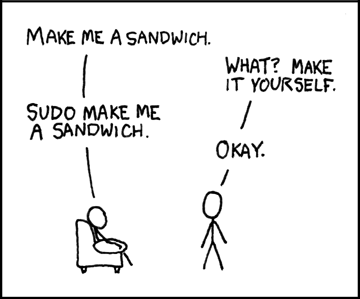
\includegraphics[height=30mm,width=30mm]{sandwich}
    \begin{quote}
      \rmfamily\textit\textbf\color{darkgray}{\large
      ``It's not a bug, its a feature.''}
      %\vskip3mm\hspace*\fill{\small--- William Shakespeare, Hamlet}
    \end{quote}
  \end{textblock}
\end{frame}
}

\begin{frame}
\tableofcontents
\end{frame}

% TODO: Refaire les schémas
% TODO: Les premiers slides de chaque thème doivent n'afficher que le titre et ensuite le corps
% TODO: Réorganiser toute la partie mémoire système:
% Peut-être que certaines partie de user-memory doivent aussi apparaitre ici:
%  Problèmatique
%  Segmentation
%  Pagination
%  Fonctionnement de la pagination
%  Fonctionnement d'un appel système
%  La séparation de la mémoire
%  Les erreurs de segmentation
%  L'overcommit
%  Le lazy loading
%  L'allocation backée sur un fichier "shared"
%  L'allocation backée sur un fichier "private" (COW)
%  Le cache
%  Le chargement des sections des ELF
%  L'allocation anonyme
%  La swap
%  Les algorithmes de remplacement de pages
%  Mlock et mlockall
%  Allocation backée sur un fichier périphérique
%  Fonctionnement d'un DMA
%  Les processus et les threads
%  La TLB
%  Les algorthmes de remplacement d'entrée dans la TLB
%  Fonctionnement de la pile (inclut fomit-pointer, etc...)
%  Fonctionnement du tas
%  Mapping de l'OS

\section{Gestion de la mémoire}

\subsection{Segmentation de la mémoire}

\begin{frame}{La MMU}
  Le temps partagé  permet de simuler que chaque tâche  est la seule à
  utiliser le CPU.

  En revanche, la mémoire est partagée entre les tâches. Ainsi, si une
  tâche A écrit par erreur sur l'espace d'une tâche B:
  \begin{itemize}
  \item  La tâche B plante
  \item  Le problème est complexe à trouver
  \item Il  n'y a  aucune moyen  pour empêcher la  tâche A  de faire
    cette action.
  \end{itemize}
\end{frame}

\begin{frame}[fragile=singleslide]{La segmentation}
  \begin{itemize}
    \item Premier mécanisme de protection
    \item Associe aux des droits aux zones de mémoire
    \item Indique au CPU  que certaines zone (appelés \emph{segments})
      de la mémoire ne doivent pas  être écrite ou ne doivent pas être
      exécutées
    \item Permet  de séparer les  données accessible en  écriture, des
      données accéssible en lecture seule, du code.
    \item Chaque section d'une binaire ELF est  chargé dans un
      segment séparé
    \item  De  nos  jours,  cette  méthode est  très  souvent  utilisé
      conjointement avec la pagination
  \end{itemize}
\end{frame}

\subsection{Pagination de la mémoire}

\begin{frame}{La pagination et la MMU}
  Les CPU  modernes intègrent  un composant appelé  MMU (\emph{Memory
    Management Unit}):
  \begin{itemize}
  \item  Unité de translation d'adresses mémoire
  \item  On parle d'adresses physiques et virtuelles
  \item Lorsque le  MMU est actif (cas nominal),  toutes les adresses
    du code assembleur sont des adresses virtuelles
  \item  Il est  possible de  configurer le  MMU avec  une instruction
    spéciale et  en lui  donnant un pointeur  sur un tableau  (dans la
    pratique,  il s'agit  plutôt d'un  arbre) associant  les adresses
    physiques et les adresses virtuelles
  \end{itemize}
\end{frame}


\begin{frame}{La MMU}
  \begin{itemize}
  \item  Il est  possible de  changer les  associations  simplement en
    chargeant fesant pointer un registre sur une autre table:
    \begin{itemize}
    \item   le  \emph{Page   Table   Base  register   (PTBR)}  ou   le
      \emph{Translation Table Base Register (TTBR))}
    \item sur Intel: CR3
    \item  sur Arm: C2
    \end{itemize}
  \item On  défini alors une table  par tâche.  Lors  du changement de
    contexte, on change aussi de table
  \item Le CPU possède alors deux modes:
    \begin{itemize}
    \item  Utilisateur
    \item  Superviseur
    \end{itemize}
  \item  Seul  le  mode  superviseur  (l'OS) permet  de  modifier  les
    associations de la MMU
  \end{itemize}
\end{frame}

\begin{frame}{La MMU}
  \begin{center}
    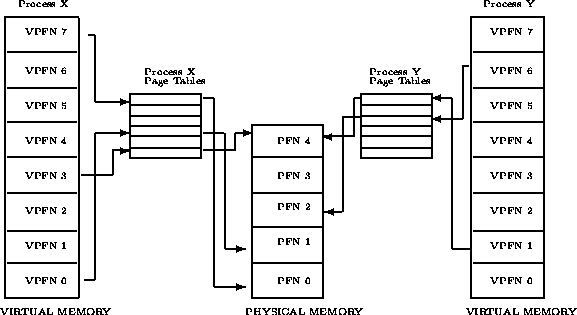
\includegraphics[height=6cm]{pics/img9}
  \end{center}
  \note{Nous verrons  par la suite comment passer  du mode superviseur
    au  mode utilisateur  et vice  versa\\}
  \note{Vérifier  sur wikipedia  ``adresse  virtuelle'' et  ``mémoire
    paginée''}
\end{frame}

\begin{frame}{La MMU}
Concretement:
  \begin{itemize}
    \item Les pages peuvent être de tailles fixe ou variables.
    \item Sous Linux,  afin de simplifier la gestion,  on utilise pour
      la plupart des architectures des pages de 4Kio.
    \item La table de page permet d'obtenir un \emph{Page Frame Number (PFN)}
    \item Le PFN correspond aux bits de poids fort de l'adresse physique
    \item  La table  de page  est décomposée  en plusieur  tables (les
      terme   proviennent   de  l'architecture   Intel   et  se   sont
      généralisés):
      \begin{itemize}
      \item Page Global Directory (PGD)
      \item Page Middle Directory (PMD)
      \item Page Table Entry (PTE)
      \end{itemize}
    \end{itemize}
\end{frame}

\begin{frame}{La pagination et la MMU}
  \begin{center}
    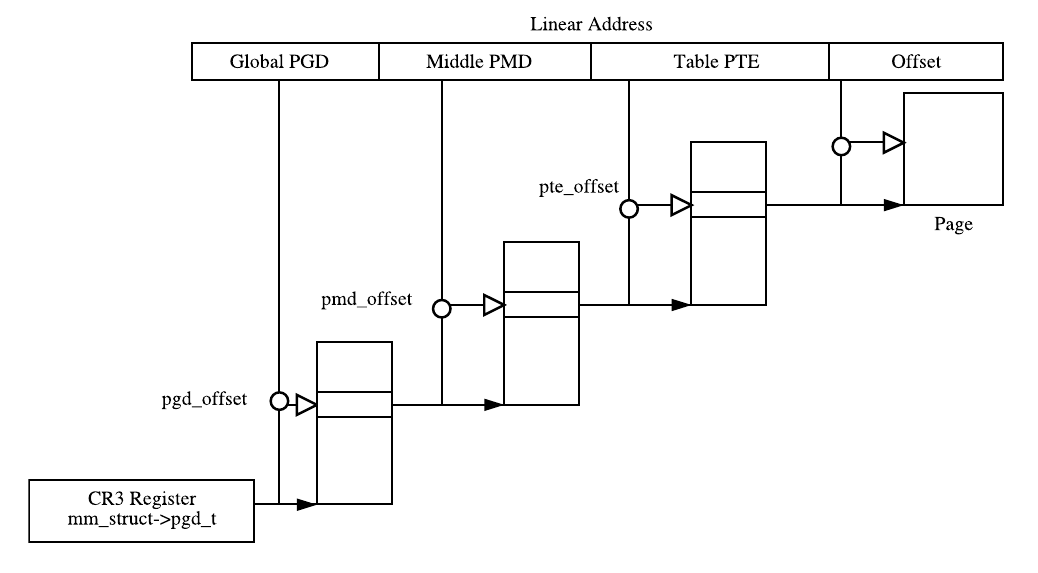
\includegraphics[height=6cm]{pics/linearaddress}
  \end{center}
\end{frame}

\begin{frame}{La pagination et la MMU}
  \begin{itemize}
      \item les tables sont aligné sur des addresse de 4K
      \item  ... Seul  les  bits  de poid  fort  (le \emph{PFN})  sont
        nécessaire pour indiquer l'emplacement de la tbale suivante en
        mémoire
      \item  ... Il  est  possible d'utiliser  les  bit restants  pour
        d'autres usages: validité de l'entrée, etc...
      \item          cf          \file{arch/asm/pgtable.h}          et
        \file{include/linux/mm-types.h}, \c{mm_struct->pgd}
    \end{itemize}
\end{frame}

\begin{frame}{La pagination et la MMU}
    \begin{center}
      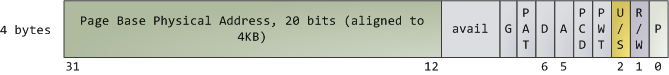
\includegraphics[width=9cm]{pics/x86PageTableEntry4KB}
    \end{center}
  \begin{itemize}
  \item R/W: Read/Write
  \item P: Present
  \item D: Dirty (souvent automatique)
  \item A: Accessed (souvent automatique)
  \item U/S: User/Supervisor
  \item avail: Available for OS usage
    \end{itemize}
\end{frame}

\begin{frame}{La MMU - gestion des exceptions}
  Toutes les adresses physiques ne sont pas associées à des adresses
  virtuelles
  \begin{itemize}
  \item Une tâche A ne peut pas accéder à la mémoire d'une tâche B
  \item Protection contre les erreurs de programmation
  \item Permet d'assurer la sécurité des systèmes multi-utilisateurs
  \item Une tâche à l'impression d'avoir toute la mémoire pour elle
  \end{itemize}
\end{frame}

\begin{frame}{La MMU - gestion des exceptions}
  Toutes  les  adresses  virtuelles  ne  sont  pas  associées  à  des
  adresses physiques
  \begin{itemize}
  \item  Lorsqu'une tâche  accède à  une adresse  non  associée.  Une
    exception est déclenchée.  Cela permet à l'OS de reprendre la main
    et de traiter l'erreur (souvent en tuant la tâche fautive)
  \item Lorsqu'une tâche souhaite allouer de la mémoire
    \begin{itemize}
    \item  La tâche demande à l'OS
    \item  L'OS choisi  un (ou  plusieurs) blocs  de  mémoire physique
      libres
    \item L'OS marque le bloc comme appartenant à la tâche
    \item  L'OS choisi un  espace d'adresse  virtuelle où  associer le
      bloc de mémoire
    \item L'OS met à jour la MMU
    \item L'OS retourne l'adresse virtuelle
    \item cf. \man{sbrk(2)} et \man{mmap(2)}
    \end{itemize}
  \end{itemize}
\end{frame}

\subsection{Passage en mode superviseur}

\begin{frame}{Passage en mode superviseur}
  Un processus utilisateur ne peut pas passer en mode superviseur.

  Comment passer en mode superviseur?
  \begin{itemize}
  \item Lorsqu'une interruption/exception est déclenchée
  \end{itemize}

  Comment appeler une fonction du système?
  \begin{itemize}
  \item  Les  tâches ont  besoin  de  faire  des demandes  au  système
    (exemple: allouer de la mémoire)
  \item Ces fonctions système s'appellent des \emph{appels système} ou
    \emph{syscall} (section 2 des pages de man)
  \item  Elles ont  très  peu de  points  communs avec  les appels  de
    fonctions classiques
  \item   Chaque  \emph{syscall}   est   associé  à   un  numéro   (cf
    \file{sys/syscall.h} \file{asm/unistd\_32.h}, \man{syscalls(2)})
  \end{itemize}

\end{frame}

\begin{frame}{Passage en mode superviseur}
  Pour utiliser les \emph{appels systèmes} (cf. \man{syscall(2)}):
  \begin{itemize}
  \item On place les arguments sur la pile
  \item On place le numéro de l'interruption sur la pile
  \item On déclenche une interruption logicielle (\c{int 0x80})
  \item  Le  CPU  passe  en  mode  superviseur  et  appelle  l'ISR  de
    l'interruption
  \item L'OS prend  la main, regarde le premier élément  de la pile et
    appelle la fonction correspondante (\file{asm-generic/unistd.h})
  \end{itemize}
  Il  existe maintenant des  instructions spéciales  sur les  CPU pour
  optimiser    les    \emph{syscall}    (instructions    \c{sysenter},
  \c{sysexit})
\end{frame}

\section{Optimisation possible grâce à la MMU}

\subsection{Les segfaults}

\begin{frame}{Gestion de la mémoire}
  Gestion des droits sur les pages
  \begin{itemize}
  \item    Il    est     possible    d'affecter    des    droits    en
    lecture/écriture/exécution sur les pages gérées par la MMU
  \item Si la tâche essaye d'écrire sur une page contenant des données
    constantes, il s'agit d'un bug et une exception est levée
  \item  On garantie  que  les pages  \emph{read-only}  ne seront  pas
    modifiées
  \item Une page contenant des données constantes (donné ou code) peut
    être mappée dans plusieurs tâches différentes
  \item ... C'est ainsi que plusieurs instance de la même bibliothèque
    ne sont chargées qu'une fois en mémoire
  \item En retirant les droits  en exécution sur les pages de données,
    on améliore la sécurité du système (impossible d'exécuter une page
    contenant des données)
  \item Une  page accessible  en écriture peut  être mappée  dans deux
    tâches afin de leur permettre de partager des données
  \item cf \file{/proc/PID/maps}
  \end{itemize}
\end{frame}

\begin{frame}{Gestion de l'espace d'adressage virtuel}
  Le MMU permet à l'OS de mieux utiliser la mémoire:
  \begin{itemize}
  \item  L'OS peut  donner  des espaces  d'addressage virtuel  contigu
    alors que la mémoire physique est fractionnée
  \item Le système n'alloue jamais la plage $[0, 1024]$
    \begin{itemize}
    \item Cela donne une plage de valeurs spéciales (ex: NULL)
    \item Ainsi, lors du debug, vous êtes certains qu'un pointeur $\in
      [0, 1024]$ est non valide
    \item En dehors des pointeurs,  les nombres que l'on manipule sont
      très  souvent <  1024.   Ce système  nous  permet de  rapidement
      repérer des casts abusifs entre des integers et des pointeurs
    \end{itemize}
  \item ``Sun a inventé le SegFault''
  \end{itemize}
\end{frame}

% Ajouter une section sur les algorithme de remplacement d'entrée dans la TLB
\begin{frame}[fragile=singleslide]{Context Swap, cache et MMU}
  \begin{itemize}
  \item  Le  MMU est  associé  à  un  cache appelé  TLB  (Translation
    lookaside buffer)
  \item  Lorsqu'une  tache tente  d'accéder  à  une  adresse, le  MMU
    regarde  le TLB,  si il  trouve l'adresse,  elle  est directement
    traduite (\emph{TLB hit})
  \item  Sinon,   il  est  nécessaire   de  traverser  la   table  des
    pages.  Cette  opération  peut   couter  une  centaine  de  cycles
    d'horloge.
  \item Il existe deux mode de fonctionnement du TLB:
    \begin{itemize}
    \item Automatique: Le MMU parcours automatique la table des pages
    \item  Manuel: Une  exception  est déclenchée.   L'OS parcourt  la
      table, met à jour le TLB et rend la main.
    \end{itemize}
    \item Notez qu'une entrée dans la TLB n'a pas la même structure qu'une entrée de PTE.
  \end{itemize}
\end{frame}

\begin{frame}[fragile=singleslide]{Context Swap, cache et MMU}
    \begin{center}
      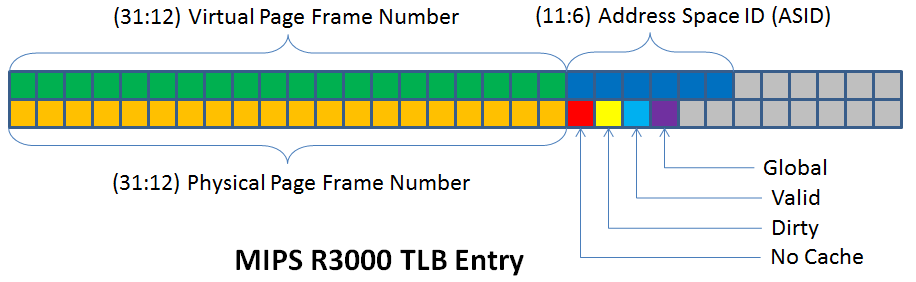
\includegraphics[width=9cm]{pics/mipsr3000_tlb}
    \end{center}
  \begin{itemize}
  \item Dans  le cas d'un  système multiprocessus, le  mappping change
    lorsque l'on passe d'une tache à l'autre
    \begin{itemize}
    \item  Certains systèmes nécessitent  d'invalider la  totalité du
      TLB
    \item  D'autre permettent  d'associer  un numéro  de  tâche à  une
      entrée  du TLB (ASID: Address Space ID). Ainsi,  lorsque la  tâche précédente  reprend la
      main, ses entrées dans le TLB sont encore valides
    \end{itemize}
  \end{itemize}
\end{frame}

\subsection{Overcommit}

\begin{frame}{Overcommit}
  Principe de l'overcommit:
  \begin{itemize}
  \item Une tâche demande une allocation
  \item Le système  enregistre la demande dans le  Memory Manager mais
    ne modifie pas le MMU
  \item  Le  système  indique   à  la  tâche  que  l'allocation  s'est
    correctement déroulée
  \item Lorsque la tâche accède à cette page, une exception est levée
  \item Le système reprend la main
  \item Il remarque qu'il avait promis cette page
  \item Il alloue un bloc physique et met à jour la MMU
  \item Il rend la main à la tâche
  \item Tout est transparent pour la tâche
  \end{itemize}
  Voir             \file{/proc/sys/vm/overcommit\_memory}            et
  \file{/proc/sys/vm/overcommit\_memory}
\end{frame}

\subsection{Mapping des fichiers en mémoire}

\begin{frame}{Gestion de la mémoire}
  Simplification des accès au IO
  \begin{itemize}
  \item   La  tâche   demande  de   mapper  un   fichier   en  mémoire
    (\man{mmap(2)})
  \item cf. \file{/proc/*/maps}
  \item  Le système  alloue un  espace d'adressage  virtuel égal  à la
    taille du fichier
  \item Le fichier en lui même n'est pas chargé en mémoire (\emph{lazy
      loading})
  \item Lorsque la  tâche accès à un espace  du fichier, une exception
    est levée et la page  demandée est chargée de manière transparente
    (\emph{on demand paging})
  \item cf. champ RSS de \file{/proc/*/smaps}
  \end{itemize}
\end{frame}

\begin{frame}[fragile=singleslide]{Les pages \emph{dirty}}
  \begin{itemize}
  \item Quelques  soit la demande de l'utilisateur,  le système marque
    les page associés à des fichier comme Read-Only.
  \item  Ainsi, lorsque  la tâche  tente  d'écrire dans  la page,  une
    exception est levée
  \item  La  page est  alors  marquée  \emph{dirty}, les  droits  en
    écriture sont données et le système rend la main
  \item (Le  marquage des page  \emph{Dirty} peut aussi  être effectué
    automatiquement par le CPU)
  \item Le système sait que  cette page devra être synchronisé avec la
    mémoire de masse
  \item Le système peut repousser cette opération
  \item Lorsque  le système  a synchroniser la  page, il la  marque de
    nouveau Read-Only
  \item Lorsque  le système  à besoin de  mémoire, il peut:
    \begin{itemize}
    \item Décharger les page readonly ou les pages \emph{clean}
    \item écrire  les pages  modifiées sur le  disque et  décharger la
      page de la mémoire
    \end{itemize}
  \item cf. champ Dirty de \file{/proc/*/smaps} et \man{free(1)}
  \end{itemize}
\end{frame}

\begin{frame}[fragile=singleslide]{Partage de page}
  \begin{itemize}
  \item Une  tâche peut demander explicitement de  partager un segment
    de mémoire avec une autre page.
  \item Il  suffit de  faire pointer deux  adresse virtuelle  vers la
    même adresse physique
  \item Lorsqu'un fichier (ou une  section du fichier) est déjà chargé
    en  mémoire,  le  système  ne  duplique  pas  la  page.  Elle  est
    automatiquement marqué comme page partagée
  \item Si  une des  tâche tente d'y  accéder en écriture,  le système
    duplique la  page juste  avant l'accès en  écriture (et  marque la
    nouvelle page comme dirty).
  \end{itemize}
\end{frame}

\subsection{La Swap}

% TODO: Ajouter une section au sujet des algorithme de remplacement de pages
% Ajouter une section au sujet des heuristiques sur l'overcommit, la swapiness, etc... : à quel moment sont déchargés ces pages
% Ajouter une section sur le OOM manager
\begin{frame}{La swap}
  \begin{itemize}
  \item La  swap est une partie  de la mémoire de  masse utilisée pour
    stockée des données de la mémoire RAM
  \item Utilisation de la Swap:
    \begin{itemize}
    \item Lorsque le système n'a plus assez de mémoire
    \item Il choisit une page physique qu'il copie sur le disque dur (parmis les pages non 'Accessed')
    \item  Il  invalide  la  page  de  la MMU  de  la  (les)  tâche(s)
      concernée(s) (le flag 'present' est suprimmé. L'OS utilise alors le PTE pour stocker l'addresse de la page dans la swap)
    \item Lorsque la  tâche accède à la page  supprimée, une exception
      est levée
    \item Le système récupère alors la page sur le disque
    \item Le système réécrit la page dans la mémoire physique
    \item  Il associe  l'adresse virtuelle  demandée avec  la nouvelle
      page physique
    \item L'OS rend la main à la tâche
    \item Tout est transparent pour la tâche
    \end{itemize}
  \item Voir \file{/proc/sys/vm/swappiness}
  \end{itemize}
\end{frame}

\begin{frame}[fragile=singleslide]{Compression de la mémoire}
  Compression de la mémoire
  \begin{itemize}
  \item  Mécanisme remplaçant  la  swap sur  les  système dépourvu  de
    mémoire  de   masse  (ou  mémoire  de  masse   limités  en  nombre
    d'écritures)
  \item  Au lieu  de copier  les page  que un  disque, les  pages sont
    compressés
  \item Mis  à part les  heuristiques utilisée, le  fonctionnement est
    identique
  \end{itemize}
\end{frame}

\begin{frame}[fragile=singleslide]{\c{mlock} et \c{mlockall}}
  \begin{itemize}
  \item Les fonctions systèmes \c{mlock} et \c{mlockall} permettent de
    demander à Linux de garder des pages (ou la totalité en mémoire)
  \item Elle empêche ainsi l'utilisation de l'overcommit et du swap.
  \item Il  ne faut  pas oublier d'allouer  une pile  suffisante avant
    d'appeler \c{mlockall} \note{Ajouter du code à ce sujet}
  \end{itemize}
\end{frame}

\begin{frame}[fragile]{Utilisation de \c{mlock}}
\begin{lstlisting}
#include <sys/mman.h>

void alloc_stack_1k() {
  char t[1024];
}

int main() {
  alloc_stack_1k();
  mlockall(MCL_CURRENT | MCL_FUTURE);
}
\end{lstlisting}
\end{frame}

\subsection{Mapping de périphérique en mémoires}

\begin{frame}{Gestion de la mémoire}
  Sécurisation des accès aux périphériques
  \begin{itemize}
  \item  Lorsque  les  registres  des  périphériques  sont  mappés  en
    mémoire, on utilise la MMU pour y accéder
  \item Il  est possible d'autoriser  l'accès à un périphérique  à une
    tâche sans lui donner d'accès au reste du système
  \item Un  système utilisant très fortement cette  méthode est appelé
    micro-kernel
  \item La méthode est peu  utilisée sous Linux (on utilisera \c{mmap}
    sur \file{/dev/mem})
  \item cf. \man{ioperm(2)}
  \end{itemize}
\end{frame}

\begin{frame}[fragile=singleslide]{\emph{mmap} sur des filedevice}
  \begin{itemize}
  \item Il est possible de  mapper en mémoire des fichier périphérique
    (avec \man{mmap(2)})
  \item  L'interprétation  de  cette  de  demande  est  laissée  à  la
    discrétion du driver
  \item Dans certains cas, ca n'a pas de sens: un port série
  \item \file{/dev/mem}:  permet de  mapper toute la  mémoire physique
    sur une adresse virtuelle
  \item  \file{/dev/video0}   (Webcam):  L'espace  de   mémoire  mappé
    représentera une frame.
  \item \file{/dev/fb0} (Frame buffer): L'espace de mémoire représente
    l'écran
  \item Ce mécanisme évite les recopies de données
  \end{itemize}
\end{frame}

\begin{frame}[fragile=singleslide]{Architecture d'un DMA}
  Un DMA \emph{Direct Memory Access}:
  \begin{itemize}
  \item Il s'agit d'un mécanisme matériel.
  \item Il doit être supporté par le contrôleur de mémoire (comprenant
    le MMU), le périphérique (ou le bus) et par l'OS
  \item  Le driver  donne au  périphérique une  adresse  (physique) où
    écrire
  \item Le périphérique demande un canal DMA au contrôleur
  \item Dans le cas d'un  PC, c'est le contrôleur PCI (le northbridge)
    qui joue le rôle de contrôleur
  \item  Le  périphérique écrit/lit  ses  données  en  passant par  le
    contrôleur de mémoire mais sans passer par le CPU
  \item Le périphérique  déclenche une interruption lorsque l'ensemble
    des données sont écrites/lues
  \end{itemize}
  Le  driver peut  décider  de  mapper la  zone  DMA directement  dans
  l'espace d'adressage de la  tâche utilisateur. Avec ce mécanisme, il
  est possible de traiter de grande quantité de données sans copie.
  \note[item]{Ajouter un shéma}
\end{frame}

\begin{frame}[fragile=singleslide]{Fonctionnement    d'un    récepteur
    satellite haut de gamme}
  \begin{itemize}
  \item Un  récepteur satellite (ou IP-TV)  est principalement composé
    d'un démodulateur/démultiplexeur et d'une carte graphique.
  \item Ces deux périphérique sont équipés de DMA
  \item  On  alloue  une  zone  de mémoire  suffisamment  grande  pour
    réceptionner quelques images (2 - 3 au moins)
  \item L'OS passe l'adresse de cette zone au démultiplexeur
  \item Des que le multiplexer à fini d'écrire une frame, il déclenche
    une interruption (et  continue d'écrire la suite dans  la suite du
    DMA)
  \item L'OS  reprend la main. Il  passe l'adresse de cette  zone à la
    carte graphique.
  \end{itemize}
  Il est ainsi possible de transférer de grande quantité de données en
  limitant l'utilisation  du CPU (et  les risque de problème  de temps
  réel)
\end{frame}

\section{Threads et Processus}

\begin{frame}{Threads}
  Thread versus Processus
  \begin{itemize}
  \item On appelle les  tâches ayant des contextes mémoires différents
    des \emph{Processus} (cf. \man{fork(2)})
  \item  Il est  possible  d'exécuter plusieurs  tâches  dans un  même
    contexte mémoire
  \item  Ces  tâche sont  appelées  \emph{threads} ou  \emph{processus
      légers} (cf. \man{clone(2)})
  \item Le fonctionnement  est alors identique au mode  sans MMU, avec
    les mêmes défauts et avantages:
    \begin{itemize}
    \item Pas  de protection contre  les erreurs de  programmation des
      autres threads
    \item Partage de l'information simplifiée
    \item Passage d'une thread à une autre beaucoup plus rapide
    \end{itemize}
  \end{itemize}
  \note{Attention au latence lors de l'allocation, et du swap}
\end{frame}

\begin{frame}[fragile]{Utilisation de processus}
\begin{lstlisting}
#include <unistd.h>

int main() {
  int r;

  r = fork();
  if (r < 0) {
     // Error
  } else if (r > 0) {
    // Parent
  } else /* r == 0 */ {
    // Child
  }
}
\end{lstlisting}
\end{frame}

\begin{frame}[fragile]{Utilisation de threads}
\begin{lstlisting}
#include <pthread.h>

void *task(void *arg) {
  int val = (int) arg;
  // Child
}

int main() {
  int arg = 42
  pthread_t id;
  pthread_create(&id, NULL, task, (void *) arg);
  // Parent
}
\end{lstlisting}
\end{frame}

\subsection{Gestion par l'OS}

\begin{frame}[fragile]{Mapping de l'OS}
  \begin{itemize}
  \item  Une  interruption  peut  avoir  lieu  depuis  n'importe  quel
    processus
  \item Lors d'une interruption (ou  d'un appel système), le CPU passe
    en mode  superviseur, mais  le mapping mémoire  reste celui  de la
    tâche d'origine
  \item Pour  des raison de performance,  il est préférable  de ne pas
    faire  de  changement de  mapping  durant  l'éxecution de  l'appel
    système (ou de l'interruption)
  \item Le noyau se trouve donc  dans une zone interdite en accès mais
    toujours mappé au même endroit quelquesoit la tâche (flag User/Supervisor).
  \item Afin  de simplifier les opérations  d'acces aux entrée/sortie,
    le  mapping du  noyau est  dit 'flat  mapping'. C'est  à  dire que
    chaque addresse  virtuelle correspond à une adresse  physique + un
    offset constant  (par défaut sur PC: \c{0xC0000000},  c'est à dire
    3Go). Cet espace s'apelle \emph{low memory}
  \end{itemize}
\end{frame}

\begin{frame}[fragile]{Mapping de l'OS}
  \begin{itemize}
  \item Le noyau peut allouer de  la mémoire en dehors de la \emph{low
      memory} (en \emph{high memory}),  mais il devrat peut-être faire
    un changement de mapping mémoire pour y accéder.
  \item  Le noyau  réserve la  \emph{low memory}  pour son  usage. Une
    tache ne peut pas allouer de la mémoire dans cette zone.
  \item Par défaut sur Linux 32bits, l'espace est partagé en 1Go / 3Go
    (Windows: 2Go / 2Go)
  \item Sur un système possédant  moins de 1Go de mémoire physique, le
    kernel  peut accéder  à  tout  l'espace physique  à  partir de  la
    \emph{low  memory}.  Sinon,  il peut  potentiellement y  avoir des
    pertes de performances  lors de l'accès par le  noyau à la mémoire
    physique supérieure au premier Gigaoctet.
  \item Une application demandant  plus de 3Go d'espace virtuelle peut
    ne pas fonctionner
  \item La solution: passer en 64bits.
  \end{itemize}
\end{frame}

\note{Montrer l'arborescence du kernel: mm, kernel, include, arch, drivers, scripts, tools, Documentation, }
